\documentclass[journal,12pt,twocolumn]{IEEEtran}

\usepackage{setspace}
\usepackage{gensymb}
\singlespacing
\usepackage[cmex10]{amsmath}

\usepackage{amsthm}

\usepackage{mathrsfs}
\usepackage{txfonts}
\usepackage{stfloats}
\usepackage{bm}
\usepackage{cite}
\usepackage{cases}
\usepackage{subfig}

\usepackage{longtable}
\usepackage{multirow}

\usepackage{enumitem}
\usepackage{mathtools}
\usepackage{steinmetz}
\usepackage{tikz}
\usepackage{circuitikz}
\usepackage{verbatim}
\usepackage{tfrupee}
\usepackage[breaklinks=true]{hyperref}
\usepackage{graphicx}
\usepackage{tkz-euclide}

\usetikzlibrary{calc,math}
\usepackage{listings}
    \usepackage{color}                                            %%
    \usepackage{array}                                            %%
    \usepackage{longtable}                                        %%
    \usepackage{calc}                                             %%
    \usepackage{multirow}                                         %%
    \usepackage{hhline}                                           %%
    \usepackage{ifthen}                                           %%
    \usepackage{lscape}     
\usepackage{multicol}
\usepackage{chngcntr}
\usepackage[utf8]{inputenc}

\DeclareMathOperator*{\Res}{Res}

\renewcommand\thesection{\arabic{section}}
\renewcommand\thesubsection{\thesection.\arabic{subsection}}
\renewcommand\thesubsubsection{\thesubsection.\arabic{subsubsection}}

\renewcommand\thesectiondis{\arabic{section}}
\renewcommand\thesubsectiondis{\thesectiondis.\arabic{subsection}}
\renewcommand\thesubsubsectiondis{\thesubsectiondis.\arabic{subsubsection}}


\hyphenation{op-tical net-works semi-conduc-tor}
\def\inputGnumericTable{}                                 %%

\lstset{
%language=C,
frame=single, 
breaklines=true,
columns=fullflexible
}
\begin{document}


\newtheorem{theorem}{Theorem}[section]
\newtheorem{problem}{Problem}
\newtheorem{proposition}{Proposition}[section]
\newtheorem{lemma}{Lemma}[section]
\newtheorem{corollary}[theorem]{Corollary}
\newtheorem{example}{Example}[section]
\newtheorem{definition}[problem]{Definition}

\newcommand{\BEQA}{\begin{eqnarray}}
\newcommand{\EEQA}{\end{eqnarray}}
\newcommand{\define}{\stackrel{\triangle}{=}}
\bibliographystyle{IEEEtran}
\raggedbottom
\setlength{\parindent}{0pt}
\providecommand{\mbf}{\mathbf}
\providecommand{\pr}[1]{\ensuremath{\Pr\left(#1\right)}}
\providecommand{\qfunc}[1]{\ensuremath{Q\left(#1\right)}}
\providecommand{\sbrak}[1]{\ensuremath{{}\left[#1\right]}}
\providecommand{\lsbrak}[1]{\ensuremath{{}\left[#1\right.}}
\providecommand{\rsbrak}[1]{\ensuremath{{}\left.#1\right]}}
\providecommand{\brak}[1]{\ensuremath{\left(#1\right)}}
\providecommand{\lbrak}[1]{\ensuremath{\left(#1\right.}}
\providecommand{\rbrak}[1]{\ensuremath{\left.#1\right)}}
\providecommand{\cbrak}[1]{\ensuremath{\left\{#1\right\}}}
\providecommand{\lcbrak}[1]{\ensuremath{\left\{#1\right.}}
\providecommand{\rcbrak}[1]{\ensuremath{\left.#1\right\}}}
\theoremstyle{remark}
\newtheorem{rem}{Remark}
\newcommand{\sgn}{\mathop{\mathrm{sgn}}}
\providecommand{\abs}[1]{\left\vert#1\right\vert}
\providecommand{\res}[1]{\Res\displaylimits_{#1}} 
\providecommand{\norm}[1]{\left\lVert#1\right\rVert}
%\providecommand{\norm}[1]{\lVert#1\rVert}
\providecommand{\mtx}[1]{\mathbf{#1}}
\providecommand{\mean}[1]{E\left[ #1 \right]}
\providecommand{\fourier}{\overset{\mathcal{F}}{ \rightleftharpoons}}
%\providecommand{\hilbert}{\overset{\mathcal{H}}{ \rightleftharpoons}}
\providecommand{\system}{\overset{\mathcal{H}}{ \longleftrightarrow}}
	%\newcommand{\solution}[2]{\textbf{Solution:}{#1}}
\newcommand{\solution}{\noindent \textbf{Solution: }}
\newcommand{\cosec}{\,\text{cosec}\,}
\providecommand{\dec}[2]{\ensuremath{\overset{#1}{\underset{#2}{\gtrless}}}}
\newcommand{\myvec}[1]{\ensuremath{\begin{pmatrix}#1\end{pmatrix}}}
\newcommand{\mydet}[1]{\ensuremath{\begin{vmatrix}#1\end{vmatrix}}}
\numberwithin{equation}{subsection}
\makeatletter
\@addtoreset{figure}{problem}
\makeatother
\let\StandardTheFigure\thefigure
\let\vec\mathbf
\renewcommand{\thefigure}{\theproblem}
\def\putbox#1#2#3{\makebox[0in][l]{\makebox[#1][l]{}\raisebox{\baselineskip}[0in][0in]{\raisebox{#2}[0in][0in]{#3}}}}
     \def\rightbox#1{\makebox[0in][r]{#1}}
     \def\centbox#1{\makebox[0in]{#1}}
     \def\topbox#1{\raisebox{-\baselineskip}[0in][0in]{#1}}
     \def\midbox#1{\raisebox{-0.5\baselineskip}[0in][0in]{#1}}
\vspace{3cm}
\title{CBSE Maths Question Paper Class10 (2009)}
\author{Dhilli Venkata Sai}
\maketitle
\newpage
\bigskip
\renewcommand{\thefigure}{\theenumi}
\renewcommand{\thetable}{\theenumi}
\renewcommand{\angle}{\measuredangle}
%
Get latex-tikz codes from 
%
\begin{lstlisting}
https://github.com/Venkatasaidhilli/IITH/tree/main/CBSE_Class10
\end{lstlisting}
\section{\textbf{Section A}}
\begin{enumerate}
\item Find the [ HCF  x LCM  ] for the numbers 100 and 190. \\
\item If 1 is a zero of the polynomial  p(x) = ax² -3(a-1)x—1, then find the value of a.\\
\item In $\triangle{LMN}$,$\angle L=50\degree$ and $\angle N=60\degree$ .If $\triangle LMN \sim \triangle PQR$ then find $\angle Q$.\\
\item If  $sec^2\theta(1 + sin\theta) (1 - sin\theta)$ = k,  then find the value of k. \\
\item If the diameter of a semicircular  protractor is 14 cm, then find its perimeter. \\
\item Find the number of solutions of the following pair of linear equations.
\begin{center}
    x + 2y - 8 = 0 \\
    2x + 4y = 16
\end{center}
\item  Find the discriminant of the quadratic equation
\begin{center}
     $3\sqrt{3}x^2+10x +\sqrt{3} = 0$ 
\end{center} 
\item If $\frac{4}{5}$, a, 2  are three consecutive terms of an A.P, then find the value of a.
\item  In Figure 1,$\triangle{ABC}$ is circumscribing a circle. Find the length of BC.
\begin{figure}[h!]
    \centering
    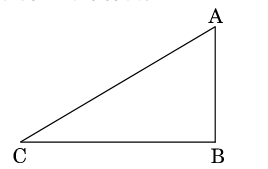
\includegraphics[width=5cm]{image1.png}
 \end{figure}
\item Two coins are tossed simultaneously. Find the probability of getting exactly one head.
\bigskip
\section{\textbf{Section B}}
\item Find all the zeroes of the polynomial $x^3 +3x^2-2x-6$ ,if two of its zeros are $-\sqrt{2}$ and $\sqrt{2}$.\\
\item Which term of the A.P.  3, 15, 27, 39, ...  will be 120 more than its $21^{st}$ term ?\\
\item In Figure 2, $\triangle ABD $ is a right triangle, right-angled at A and $AC \perp BD$. Prove that\\ $AB^2  = BC .BD$ .
\begin{figure}[h!]
    \centering
    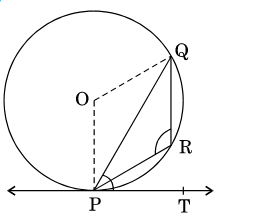
\includegraphics[width=5cm]{image2.png}
 \end{figure}
\item If  $cot\theta$= $\frac{15}{8}$ then evaluate $\frac{(2+2sin\theta)(1-sin\theta)}{(1+cos\theta)(2-2cos\theta)}$ \begin{center}
    OR 
\end{center}
\\ Find the value of tan 60°, geometrically.\\
\item If  the  points  A (4, 3) and  B (x, 5)  are on the circle with the centre O (2, 3), find the value of x
\bigskip
\section{\textbf{Section C}}
\item Prove that $3+\sqrt{2}$ is a irrational number.\\
\item Solve for x and y:
\begin{equation}
     \frac{ax}{b}- \frac{by}{a} = a+b\\ \nonumber
\end{equation}
\begin{equation}
    ax-by = 2ab \nonumber
\end{equation}
\item The sum of first six terms of an arithmetic progression is 42. The ratio of its $10^{th}$ term to its $30^{th}$ term is 1:3. Calculate the first and the thirteenth term of the A.P.\\
\item evaluate:
\begin{center}
    $\frac{2}{3}cosec^2 58\degree - \frac{2}{3}cot58\degree tan32\degree - \frac{5}{3}tan13\degree tan37\degree tan45\degree tan53\degree tan77\degree $
\end{center}
\\ 
\item Draw a right triangle in which sides (other than hypotenuse) are of lengths 8 cm and 6 cm. Then construct another triangle whose sides are $\frac{3}{4}$ times the corresponding sides of the first triangle.\\
\item In  Figure 3,  $AD \perp BC$ and BD = $\frac{1}{3}$ .Prove that $2CA^2 =2AB^2+BC^2$.
\begin{figure}[h!]
    \centering
    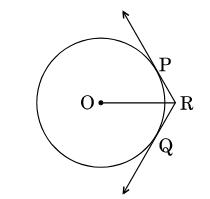
\includegraphics[width=5cm]{image3.png}
 \end{figure}
\begin{center}
    OR
\end{center}
 In  Figure  4,  M  is  mid-point  of  side  CD  of  a  parallelogram  ABCD. The line BM  is  drawn  
intersecting  AC  at L  and AD  produced  at E. Prove that  EL  = 2 BL.
\begin{figure}[h!]
    \centering
    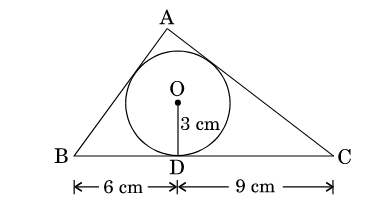
\includegraphics[width=5cm]{image4.png}
 \end{figure}
\item Find the ratio in which the point (2, y) divides the line segment joining the points A (-2, 2) and B (3, 7). Also find the value of y. \\
\item Find the area of the quadrilateral ABCD whose vertices are A (-4, -2),B (-3, -5), C (3, -2) and D (2, 3). \\
\item The area of an equilateral triangle is $49\sqrt{3} cm^2$. Taking each angular point as centre, circles are drawn with radius equal to half the length of the side of the triangle. Find the area of triangle not included in the circles. [Take $\sqrt{3}$ = 1.73]
\begin{center}
    OR
\end{center}
 Figure 5 shows a decorative block which is made of two solids — a cube and a hemisphere. The base of the  block is a cube with edge 5 cm and the hemisphere, fixed on the  top, has a diameter of 4.2 cm. Find the total surface area of the block. [Take $\pi$ = $\frac{22}{7} $]
\begin{figure}[h!]
    \centering
    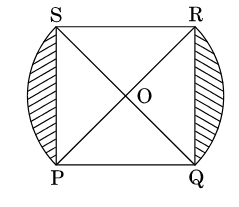
\includegraphics[width=5cm]{image5.png}
 \end{figure}
\item  Two dice are thrown simultaneously. What is the probability that
\begin{enumerate}
    (i)   5 will not come up on either of them ?\\
    (ii)  5 will come up on at least one ?\\
    (iii) 5 will come up at both dice ?\\
\end{enumerate}
\section{\textbf{Section D}}
\item Solve the following equation for x :
\begin{equation}
    9x^2 - 9(a+b)x + (2a^2+5ab+2b^2) = 0 \nonumber
\end{equation}
\begin{center}
    OR
\end{center}
If (-5) is a root of the quadratic equation $2x^2 + px -15  =  0$ and the quadratic equation  $p(x^2 + x) + k = 0 $ has equal roots, then find the values of p and k.\\
\item Prove that the lengths of the tangents drawn from an external point to a circle are equal.
Using the above theorem prove that :\\
If quadrilateral ABCD is circumscribing a circle, then\\
AB + CD = AD + BC. \\
\item An  aeroplane  when  flying  at  a  height  of  3125  m  from  the  ground passes vertically below another plane at an instant when the angles of elevation of the two planes from the same point on the ground are 30\degree and 60\degree respectively. Find the distance between the two planes at that instant.
\item A juice seller serves his customers using a glass as shown in Figure 6. The inner diameter of the cylindrical glass is 5 cm, but the bottom of the glass has a hemispherical portion raised which reduces the capacity of  the  glass.  If  the  height  of the  glass  is  10  cm,  find  the  apparent capacity of the glass and its actual capacity. (Use $\pi$ = 3.14)
\begin{figure}[h!]
    \centering
    \includegraphics[width=5cm]{image6.png}
 \end{figure}
\begin{center}
OR
\end{center}
A cylindrical vessel with internal diameter 10 cm and height 10 5 cm is full of water. A solid cone of base diameter 7 cm and height 6 cm is completely immersed in water. Find the volume of
\begin{enumerate}
    (i) water displaced out of the cylindrical vessel.\\
    (ii) water left in the cylindrical vessel.
\end{enumerate}
[Take $\pi$ = $\frac{22}{7}$] \\
\item  During the medical check-up of 35 students of a class their weights were recorded as follows :
\begin{center}
        \begin{tabular}{ c c c }
            \underline{Weight(in kg)} & \underline{Number of students}  \\
            38-40 & 3  \\
            40-42 & 2  \\
            42-44 & 4  \\
            44-46 & 5  \\
            46-48 & 14 \\
            48-50 & 4  \\
            50-52 & 3  \\
        \end{tabular}
    \end{center}
\end{enumerate}
\end{document}
